\documentclass[runningheads]{llncs}
\usepackage{graphicx} % Required for inserting images
\usepackage{amsmath,amssymb,amsfonts}
\usepackage{algorithmic}
\usepackage{textcomp}
\usepackage{float}
\usepackage{etoolbox}
\usepackage{hyperref}
\usepackage{hyperref}
\usepackage{tikz}
\usepackage{fontawesome}
\usepackage{caption}
\usepackage{url}
\usepackage{listings}
\usepackage{pdfpages}
\usepackage[english]{babel}
\usepackage{scalerel}
\usepackage{xcolor,colortbl}
\usepackage{cite}
\usepackage[linesnumbered,ruled,vlined]{algorithm2e}
\usepackage{amsmath}
\usepackage{amssymb}
\usepackage{multirow}


\title{A Voter-to-Voter Internet Voting Protocol with Federated Distributed Key Generation}
\author{Stanislaw Baranski\inst{1}}
\institute{Gdansk University of Technology, Narutowicza 11/12 80-233, Gdansk, Poland \email{stanislaw.baranski@pg.edu.pl}}

\begin{document}

\maketitle


\begin{abstract}
This paper presents a voter-to-voter Internet voting protocol that uses a novel technique called Federated Distributed Key Generation (FDKG), which allows dynamic participation in the key generation process, ensuring robustness against node unavailability and enabling a flexible trust model among participants. The protocol can be implemented in a peer-to-peer environment with zero transaction fees, a significant advantage over protocols that require either a hosting fee or a per-vote fee. The protocol uses threshold cryptography, which ensures that a subset of nodes can decrypt voting results, preventing any single node from blocking the voting process. Using zero-knowledge proofs (zkSNARKs), the protocol guarantees the integrity and privacy of the voting process, allowing voters to verify the correctness of the process without compromising their anonymity. The paper also discusses the protocol's resilience to Byzantine nodes and its application to small-scale voting where participants know each other, making it particularly suitable for governance models such as non-government organizations, corporate boardrooms, homeowners' associations, and open-source projects. The protocol is rigorously analysed for security, decipherability and privacy, and experimental results demonstrate its practical feasibility and scalability. This work contributes to a significant advancement in trust models for secure and decentralised voting protocols.
\end{abstract}

\keywords{Internet Voting \and Digital Democracy \and Federated Distributed Key Generation \and Threshold Cryptography \and  zkSNARKs \and Blockchain}

\section{Introduction}

Voting serves as a fundamental mechanism for collective decision-making, employed across diverse contexts ranging from non-government organizations and corporate boardrooms to domestic presidential elections and global online polls.

The methodologies of voting vary widely, encompassing traditional paper-based voting, mail-in ballots, electronic systems such as direct-recording electronic (DRE) machines, and internet-based voting processes \cite{parkGoingBadWorse2021}.

As articulated by Vitalik Buterin \cite{buterinBlockchainVotingOverrated2021}, each voting system encounters a trilemma, necessitating a choice between two of three critical attributes:

\begin{itemize}
\item \textbf{Democratic}: Ensuring equitable and accessible participation for all eligible voters.
\item \textbf{Secure}: Guaranteeing the integrity, transparency, privacy, and resilience against potential threats.
\item \textbf{Efficient}: Achieving simplicity, speed, and cost-effectiveness in the voting process.
\end{itemize}

In conventional political elections, the emphasis on security and democracy often leads to a compromise on efficiency. Conversely, social media polls prioritize democracy and efficiency, but at the cost of security. The market system exemplifies an efficient and secure decision-making model, where consumer choices influence corporate power. However, it lacks democratic inclusivity, rendering it unsuitable for public goods decision-making.

The inherent inefficiencies in traditional voting methods result in substantial costs and infrequent election cycles, typically ranging from annual to once every six years \cite{buterinBlockchainVotingOverrated2021}.

Internet voting (i-voting) emerges as a seemingly ideal solution, paralleling the widespread adoption of online banking. Particularly during events like the COVID-19 pandemic, i-voting presents as a conventional, cost-effective, swift, and safe alternative. Its potential to enhance voter turnout, increase the frequency of elections, and facilitate various democratic models such as direct democracy, liquid democracy, and alternative voting systems is significant \cite{laslierLoserPluralityVoting2011}.

Furthermore, the evolution of smart cities, crypto cities \cite{buterinCryptoCities2021}, Decentralized Autonomous Organizations (DAOs) \cite{wangDecentralizedAutonomousOrganizations2019}, and other algorithmic governance models \cite{GovernmentAlgorithm2022} are intrinsically linked to the advancement of electronic voting systems. Despite the pressing need for such systems, as evidenced in countries like Switzerland \cite{ElectronicVotingSwitzerland2023} and Estonia \cite{ElectronicVotingEstonia2023}, the global progress in adopting these modern democratic tools lags behind other digital transformations, such as online banking.

The feasibility of internet voting has been a subject of extensive research, particularly in the field of cryptography, a critical aspect of system security. However, skepticism persists regarding the viability of public internet voting \cite{parkGoingBadWorse2021, mearianWhyBlockchainbasedVoting2019, shanklandNoBlockchainIsn2018, leeBlockchainbasedElectionsWould2018, schneierBlockchainVoting2020, schneierBlockchainTrust2019}. In Germany, for instance, e-voting development ceased following a judicial ruling against electronic voting machines, citing their contradiction to the public nature of elections \cite{ElectronicVotingCountry2023}. The reluctance towards e-voting stems from technology trust issues and the reliance on authoritative control over the voting process.

Criticism of internet voting predominantly revolves around two arguments:

\begin{enumerate}
\item The inherent imperfection of software, which precludes absolute trust.
\item Excessive reliance on authorities overseeing the voting process.
\end{enumerate}

Recent research by MIT scholars posits that any paperless voting system is inherently flawed \cite{parkGoingBadWorse2021}. Notably, even high-quality software, ranking in the 90th percentile within the industry, contains an average of one defect per ten thousand lines of code \cite{llaguno2017CoverityScan2017}. These defects can lead to either malfunctions or exploitable vulnerabilities, potentially compromising the voting process. The critical concern is that software flaws should not precipitate undetectable alterations in election outcomes, a guarantee seemingly unattainable given the nature of software development.
Recent developments in cryptography, particularly zero-knowledge proofs, offer promising solutions to ensure the integrity of voting software \cite{parnoPinocchioNearlyPractical2013}. Zero-knowledge proofs enable public verification of the voting process's correctness without compromising voter privacy. This approach, utilizing cryptographic verification, aligns with the software independence requirement outlined in \cite{parkGoingBadWorse2021}, allowing for third-party verification without relying on the voting system's internal software.

However, trust in the software is only part of the equation; the reliability of the hardware used by voters is also crucial. Critics argue that the security of internet voting protocols depends on the assumption that voter devices are uncompromised and function as intended, a premise often considered unrealistic \cite{parkGoingBadWorse2021}. Despite vulnerabilities in hardware, including trusted platforms like Intel® Software Guard Extensions \cite{mckeenIntelSoftwareGuard2016} that have been compromised \cite{goodinIntelSGXVulnerable2020, IntelSGXBroken2019, bulckForeshadowExtractingKeys}, there is a trend towards enhancing hardware security. Notably, smartphones are increasingly equipped with Trusted Execution Environments (TEE), such as Apple's Secure Enclaves \cite{SecureEnclave}, Samsung's Knox \cite{kanonovSecureContainersAndroid2016}, HTC's Zion \cite{exodusZION}, and ARM's TrustZone \cite{ARMSecurityTechnology}. These developments suggest a positive trajectory in cybersecurity \cite{golombBelieveItCybersecurity2018}.

Moreover, Appel et al. \cite{appelEvidenceBasedElectionsCreate2019} highlight that no vote counting method is infallible, whether it be optical scanning, touchscreen systems, or manual counting. The critical issue is not the absence of security but rather the degree of security and the nature of trust assumptions involved.

The second major critique of internet voting centers around the trust placed in authorities overseeing the process. Traditional polling stations, being physically accessible and observable, offer a form of evidence-based trust that digital polling stations—servers—lack \cite{starkEvidenceBasedElections2012}. The principle of evidence-based elections requires not just determining the true winner but also providing convincing evidence of this outcome to the electorate \cite{appelEvidenceBasedElectionsCreate2019}. This evidence is deemed convincing when the voting process is both auditable and audited; it must generate a reliable audit trail and routinely execute this audit as part of the voting process.

\textbf{Ideally, the voting process should be completely trustless, meaning that, there should be no trust assumptions other than in our perception.}

In reality, the complete monitoring of elections is impractical, leading to a reliance on designated staff to oversee the process. This approach aligns with the $1 \textrm{ of } N$ trust model, where the system's integrity depends on at least one honest observer among $N$ being present to report any discrepancies \cite{buterinTrustModels2020}. However, as the number of observers diminishes, the likelihood of having at least one honest observer decreases, thereby compromising the trustworthiness of the election. Consequently, a robust voting process should involve a large, diverse group of observers—the greater the $N$, the more credible the process.
Criticism of centralized internet voting systems often centers on their reliance on a stringent $1\textrm{ of }1$ trust model. This model implies a single point of failure: the central authority. If this authority is compromised, the entire trust in the system collapses, as it fails to provide convincing evidence of the software's correctness to the electorate.

In response to this critique, two counterarguments emerge:
\begin{enumerate}
\item The first counterargument posits that even in the absence of trust in organizers, the requirement for them to generate cryptographic proof of vote tallying ensures accuracy. Any discrepancy in the results would be detectable during the verification of this proof.
\item The second counterargument suggests decentralizing the traditional centralized authority. This can be achieved through distributed systems and consensus mechanisms, transforming the trust model from $1 \textrm{ of } 1$ to more robust models. These include $N \textrm{ of } N$, where all participants must function correctly; $Few \textrm{ of } N$, where a subset of nodes must be reliable; or $\frac{N}{2} \textrm{ of } N$, where the system remains functional as long as a majority of the nodes operate correctly.
\end{enumerate}

When trust assumptions in these systems are violated, different properties may fail, such as liveness, safety, censorship-resistance, privacy, or correctness.

Blockchain technology has gained prominence in decentralizing trust, offering inherent guarantees of immutability, verifiability, integrity, and resistance to censorship. Consequently, blockchain has become a popular foundation for developing trust-minimizing platforms, including internet voting protocols.

Even in scenarios where blockchain is not utilized, and instead, a distributed set of authorities (referred to as Guardians) administer the voting system—as seen in Helios~\cite{adidaHeliosWebbasedOpenAudit2008} or ElectionGuard~\cite{ElectionGuard}—the challenge of involving external organizers remains. These systems still necessitate a mechanism to ensure that the guardians themselves are trustworthy and that their collective actions yield a reliable and verifiable election outcome.

In this paper, we introduce a novel peer-to-peer voting protocol, employing a generalized trust model that empowers participants to autonomously select their trusted guardians within the system. 

Figure~\ref{fig:trust-models} illustrates the evolution of internet voting trust models, progressing from reliance on a singular trusted third party to distributed third parties, and culminating in the peer-to-peer and delegated voter-to-voter models that we explore herein.

\begin{figure}
    \centering
    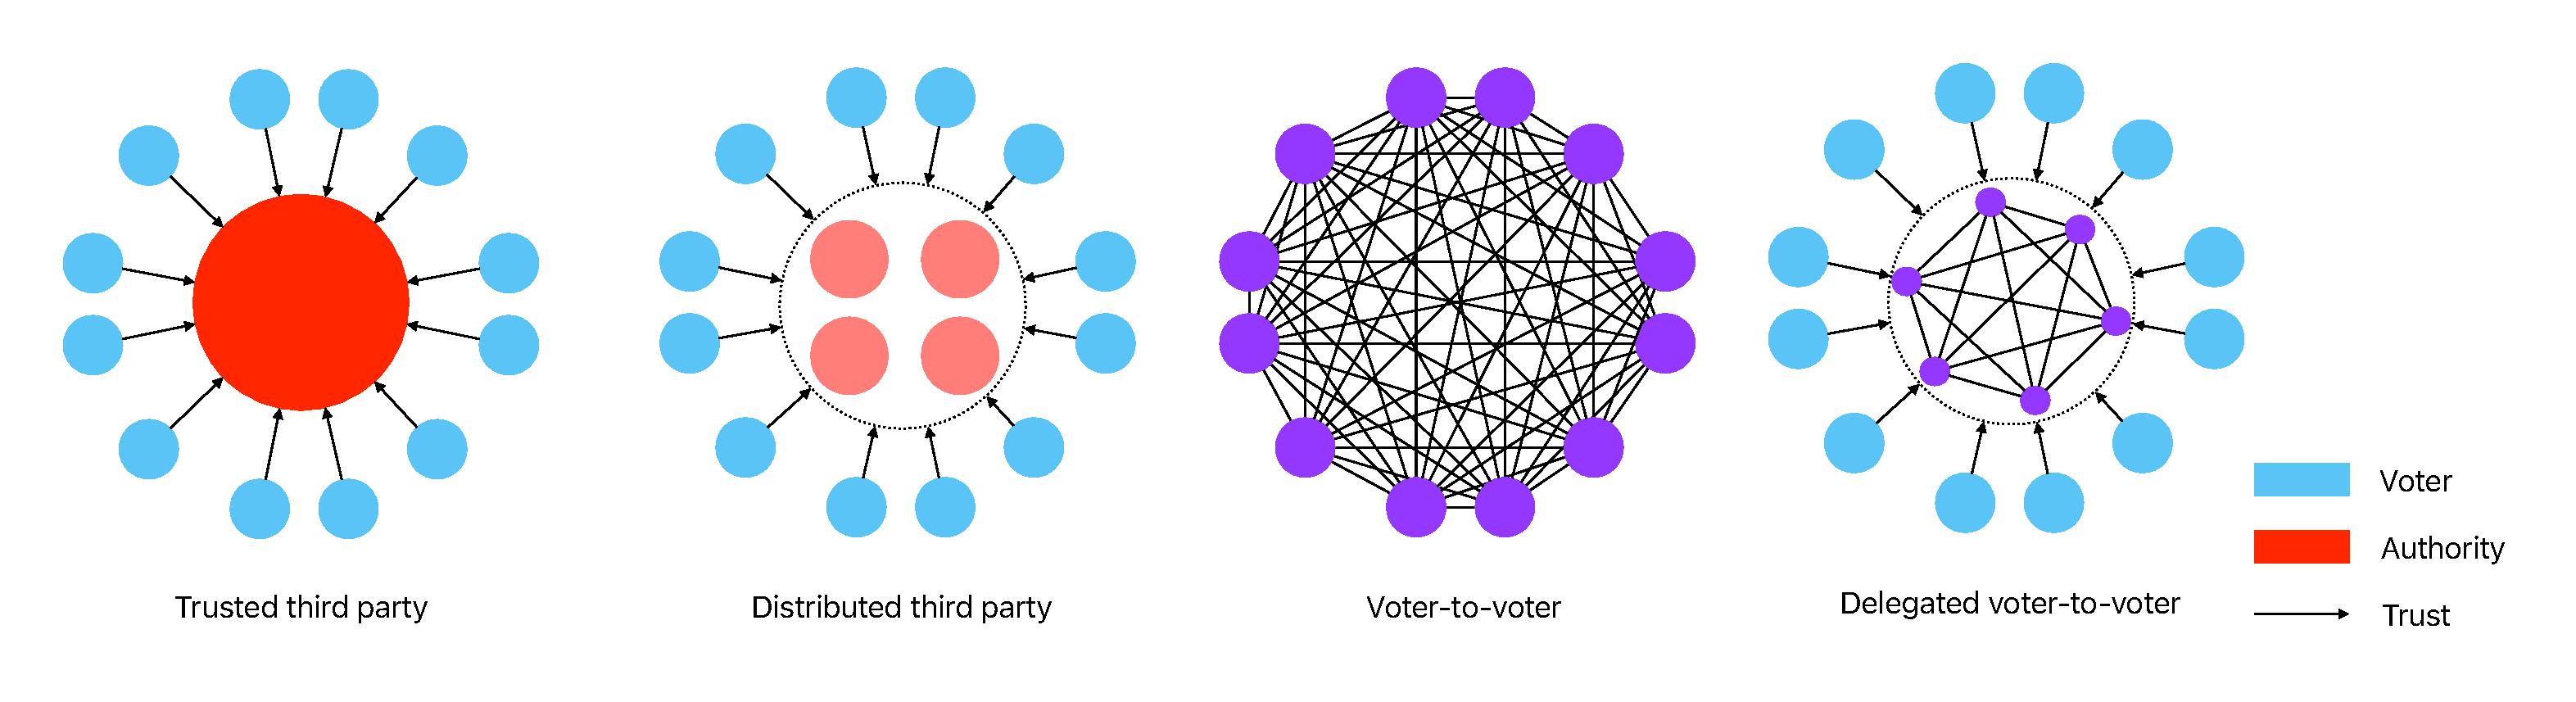
\includegraphics[width=\textwidth]{trust-models-voting.pdf}
    \caption{Four trust models: trusted third party, distributed authorities, peer-to-peer, delegated voter-to-voter}
    \label{fig:trust-models}
\end{figure}

Protocols employing a distributed set of authorities typically leverage Distributed Key Generation (DKG) \cite{gennaroSecureDistributedKey1999} to allocate keys among participants. The integrity of the voting process is maintained under the assumption of an 'honest majority', where privacy is preserved provided there is no collusion among parties. However, the conventional DKG model faces challenges in voting systems, particularly when parties involved in the DKG are unavailable, potentially disrupting the voting process \cite{haoAnonymousVotingTworound2010}. While some methods use collateral deposits to incentivize participation \cite{elsheikhDisputefreeScalableOpen2022}, we find this approach impractical for broader applications. Instead, we propose a protocol based on threshold cryptography, which tolerates a certain level of node unavailability. Our contributions are as follows:

\begin{enumerate}
    \item We introduce an innovative internet voting protocol based on a delegated voter-to-voter trust model. This model reflects the trust relationships within a group, translating them into the system’s security and availability features. It is particularly apt for small-scale elections where participants are familiar with each other and existing trust lines are well-established.
    
    \item We develop a new technique for Dynamic Distributed Key Generation (DKG), termed Federated DKG (FDKG). FDKG facilitates joint key-pair establishment by members with a single message exchange, without prior knowledge of all participants.
            
    \item We detail a practical implementation strategy for a peer-to-peer environment with no transaction fees, and an alternative public blockchain implementation using a single paymaster. This approach offers a significant advantage over existing protocols that require hosting or per-vote fees.

    \item We present an open-source implementation of our protocol in TypeScript and Golang, enhancing its adaptability across various platforms and thereby expanding its accessibility and practical utility.
    
    \item We propose a novel solution to address the issue of node unavailability, which can hinder the election process. By employing threshold cryptography and the concept of Guardian Sets, each participant divides their secret among a selected group of trusted nodes. Assuming these Guardian Sets consist of reputable and reliable network members, the risk of failure or collusion is minimized. This ensures that our protocol’s improved availability does not compromise its security.
\end{enumerate}


\section{Related Work}

Internet voting protocols commonly depend on a trusted third party, with variations in server capabilities determining integrity, anonymity, privacy, censorship-resistance and coercion resistance based on the trustworthiness of this entity. Current research predominantly employs blockchain technology for its integrity and transparency in vote storage, as seen in systems like Voatz, Polys, Follow My Vote, Verify-Your-Vote, OpenVoteNetwork, TIVI, Stellot, Cicida, and MACI \cite{mooreWestVirginiaMobile2019, PolysOnlineVoting, SecureDecentralizedApplication2023, chaiebVerifyYourVoteVerifiableBlockchainBased2019, haoAnonymousVotingTworound2010, mccorrySmartContractBoardroom2017, seifelnasrScalableOpenVoteNetwork2020, elsheikhDisputefreeScalableOpen2022, TIVIPoweredSmartmatic, NowYouCan2016, baranskiPracticalIVotingStellar2020, BuildingCicadaPrivate, A16zCicada2023, ethereumfoundationMinimalAntiCollusionInfrastructure2022, PrivacyscalingexplorationsMaci2023}.

Alternatively, projects like Helios, Civitas, Swisspost/Scytl, iVoting, and ElectionGuard utilize distributed authorities and Multi-Party Computation (MPC) protocols without explicitly depending on blockchain technology \cite{adidaHeliosWebbasedOpenAudit2008, clarksonCivitasSecureVoting2008, roenneJCJImprovedVerifiability2016, ElectionGuard}. These systems are not fully decentralized, relying on a closed set of trusted entities known as Guardians.

Public blockchain-based solutions typically struggle with user-friendliness and require voters to bear transaction fees. Non-blockchain solutions either work in SaaS model or as a self-hosting software moving the operational burden on election organisers potentially creating accessibility barriers for small-scale votings and non-technical operators. Hybrid systems like MACI function on both a blockchain network and a single coordinator server \cite{ethereumfoundationMinimalAntiCollusionInfrastructure2022, PrivacyscalingexplorationsMaci2023}.

Solutions based on public blockchains often face challenges in terms of user-friendliness and typically require voters to incur transaction fees, which may deter participation. In contrast, non-blockchain solutions, operating either as Software as a Service (SaaS) or self-hosted software, shift the operational burden onto election organizers. This shift can create significant accessibility barriers, particularly for small-scale voting events and organizers lacking technical expertise. Hybrid systems like MACI operate utilizing both a blockchain network and a centralized coordinator server, combining elements of decentralization with centralized control \cite{ethereumfoundationMinimalAntiCollusionInfrastructure2022, PrivacyscalingexplorationsMaci2023}.

Our proposed solution differs significantly from these models. It is free of charge, unlike public-blockchain-based systems, potentially improving voter turnout. In contrast to private-blockchain-based systems, our protocol operates without centralized servers, making it particularly suitable for smaller, informal voting contexts. This approach shifts the trust paradigm from central authorities to the voters themselves.


\newcommand{\fullmoon}{\tikz\filldraw[fill=black] (0,0) circle (0.5em);}
\newcommand{\newmoon}{\tikz\draw (0,0) circle (0.5em);}
\newcommand{\rightmoon}{\tikz\draw (0,0) circle (0.5em); \filldraw[fill=black] (0,0) arc (90:270:0.5em) -- cycle;}
\newcommand{\leftmoon}{\tikz\draw (0,0) circle (0.5em); \filldraw[fill=black] (0,0) arc (270:90:0.5em) -- cycle;}
\newcommand{\halfmoon}{\tikz\draw (0,0) circle (0.5em); \filldraw[fill=black] (0,-0.5em) rectangle (0,0.5em);}


\begin{table*}[!h]
\centering
\newcommand{\YES}{\cellcolor{red!50}Yes}
\newcommand{\NO}{\cellcolor{green!50}No}
\begin{tabular}{p{0.2\textwidth}p{0.2\textwidth}p{0.17\textwidth}p{0.17\textwidth}p{0.21\textwidth}}
\noalign{\smallskip}\hline\noalign{\smallskip}
\textbf{Property} & \textbf{Centralised server} & \textbf{Private network} & \textbf{Public blockchain} & \textbf{Voter-to-Voter network}\\
\noalign{\smallskip}\hline\noalign{\smallskip}
Transaction fees & \NO & \NO & \YES & \NO \\
\hline
Service costs\footnote{The cost of service includes all costs related to implementation, maintenance, and fees} & \cellcolor{yellow!50} Medium & \cellcolor{red!50} High & \cellcolor{green!50} No  & \cellcolor{green!50} No \\
\hline
User-Friendliness & \cellcolor{green!50} High & \cellcolor{green!50}High & \cellcolor{red!50} Low & \cellcolor{yellow!50} Medium \\
\hline
Trust to\footnote{Trust is a broad term that refers to different properties of the system, but most of the time it answers the question of who holds the properties of censorship-resistance, privacy, and/or correctness.} & \cellcolor{red!50} Central authority & \cellcolor{yellow!50} Authorities\footnote{Examples of authorities are: "Election Officials, Trustees Canvass Board Members, Government Officials or other trusted authorities who are responsible and accountable for conducting the election", \href{http://www.electionguard.vote/basics/steps/1_Key_Ceremony/}{source}.} & \cellcolor{yellow!50} Miners & \cellcolor{yellow!50} Voters  \\
\noalign{\smallskip}\hline
\hline
\end{tabular}

\caption{A comparative analysis of four types of Internet voting protocols: centralised server, public blockchain-based, private infrastructure-based, and voter-to-voter network-based, highlighting their differences in transaction fees, service costs, user-friendliness, and trust dynamics, where trust refers to an entity that guarantees properties of censorship resistance, privacy, and/or correctness. Service costs include all costs related to implementation, maintenance and fees.}
\label{table-comparision}

\end{table*}

Moreover, different systems achieve varying security and privacy properties based on their underlying assumptions. For instance, OpenVoteNetwork eliminates the need for trusted third parties by adopting a self-tally scheme, ensuring perfect ballot secrecy but is susceptible to denial of service attacks \cite{haoAnonymousVotingTworound2010, mccorrySmartContractBoardroom2017, seifelnasrScalableOpenVoteNetwork2020, elsheikhDisputefreeScalableOpen2022}. Cicida achieves voter anonymity using homomorphic time-lock puzzles combined with Semaphore for zero-knowledge set membership proofs \cite{BuildingCicadaPrivate, A16zCicada2023}. MACI, offering coercion-resistance, relies on a single coordinator server for ballot privacy \cite{ethereumfoundationMinimalAntiCollusionInfrastructure2022, PrivacyscalingexplorationsMaci2023}.

ElectionGuard distributes encryption keys among Guardians, using Distributed Key Generation and multi-party computation for decryption, with a quorum parameter to ensure completion even if some Guardians are absent \cite{ElectionGuard}.

Our protocol parallels ElectionGuard's approach but extends it by allowing every voter to act as a Guardian, sharing their secret input with trusted parties instead of the entire network. This model not only decentralizes trust further but also enhances privacy and security by distributing the power of vote verification among a wider set of participants.


\paragraph{Objectives}
In designing the protocol, we focused on key objectives to meet the essential challenges and needs of a secure and practical internet voting protocol. These objectives are:

\begin{enumerate}
    \item \textbf{Distributed Model}. Use a completely distributed model to eliminate the need for central authorities or trusted intermediaries. This approach increases the system's resilience to attacks and reduces the risk of having single points of failure.
    \item \textbf{Flexible trust.} Use a social mapping approach for security, where the system relies on the structure of trust within the community. People that are more trusted should have a bigger role in maintaining security.
    \item \textbf{Privacy.} Ensure strong privacy for voter identity and choices, using cryptographic methods based on the honest-majority assumption. This means individual votes remain secret and cannot be decrypted unless the most important nodes collude.
    \item \textbf{Robustness}: The protocol should be resilient to partial participation, particularly in the final round, allowing for flexible involvement without compromising the voting process integrity.
    \item \textbf{Accessibility.} Ensure the protocol works smoothly on common devices like smartphones and laptops. This makes it accessible, scalable, and easy to use for everyone.
\end{enumerate}


% Party
\newcommand{\PartySecretKey}[1]{\ensuremath{s_{#1}}}
\newcommand{\Party}[1]{\ensuremath{P_{#1}}}
\newcommand{\Parties}{\ensuremath{\mathbb{P}}}
\newcommand{\VotesSize}{\ensuremath{|\mathbb{V}}|}

% Voting keys
\newcommand{\EncryptionKey}{\textbf{E}}
\newcommand{\DecryptionKey}{\textbf{d}}

% Partial voting keys
\newcommand{\PartialDecryptionKey}[1]{\ensuremath{d_{#1}}}
\newcommand{\PartialEncryptionKey}[1]{\ensuremath{E_{#1}}}

% Ciphertexts
\newcommand{\EncryptedPartialDecryptionKeyShare}[2]{\ensuremath{C_{#1,#2}}}
\newcommand{\SetOfEncryptedPartialDecryptionKeys}{\ensuremath{\mathbb{C}}}
\newcommand{\SetOfFDKG}{\ensuremath{\mathbb{D}}}
\newcommand{\SetOfSharesOfPartialDecryption}{\ensuremath{\mathbb{C}}}

% Shares
\newcommand{\IthDecryptionKey}[1]{\ensuremath{d_{#1}}}
\newcommand{\IthEncryptionKey}[1]{E_{#1}}

% Private channel
\newcommand{\DecryptionUsingOf}[2]{\ensuremath{\texttt{Dec}_{#1}(#2)}}
\newcommand{\EncryptionUsingOf}[2]{\ensuremath{\texttt{Enc}_{#1}(#2)}}

\newcommand{\PartialDecryptionKeyShare}[2]{\ensuremath{[d_{#1}]_{#2}}}


\newcommand{\ProofFDKG}[1]{\ensuremath{\textrm{PROOF}_{#1,\textrm{FDKG}}}}

\newcommand{\ProofFDKGInformal}{"Given \PartialEncryptionKey{i}, \EncryptedPartialDecryptionKeyShare{i}{j} and $\Party{j} \in \GuardianSetOf{i}$, I know $f_i = a_0, \dots, a_{t-1}$, $r1_1,\dots,r1_k$, and $r2_1,\dots,r2_k$, s.t. $\PartialEncryptionKey{i}=a_0G$ and the \EncryptedPartialDecryptionKeyShare{i}{j} is an encrypted value of a polynomial $f_i(\cdot)$ applied to $j$"}

\newcommand{\ProofBALLOT}[1]{\ensuremath{\textrm{PROOF}_{#1,\textrm{BALLOT}}}}

\newcommand{\ProofBALLOTInformal}{"Given \EncryptionKey{} and \Ballot{i} = $(C1, C2)$, I know \BlindingFactor{i}, and \Vote{i} s.t. $\Vote{i} \in \{2^0, 2^j, \ldots, 2^{(l-1)j}\}$ and $\Ballot{i} = (\BlindingFactor{i} G,\ \BlindingFactor{i} \EncryptionKey{} + \Vote{i})$"}

\newcommand{\ProofPD}[1]{\ensuremath{\textrm{PROOF}_{#1,\textrm{PD}}}}

\newcommand{\ProofPDInformal}{"Given $\TotalA{}, \PartialDecryptionFrom{i}, \PartialEncryptionKey{i}$, I know a partial decryption key $\PartialDecryptionKey{i}$ s.t. $\PartialEncryptionKey{i} = \PartialDecryptionKey{i} \cdot G$ and $\PartialDecryptionFrom{i} = \PartialDecryptionKey{i} \cdot \TotalA{}$"}

\newcommand{\ProofPDS}[2]{\ensuremath{\textrm{PROOF}_{#1,#2,\textrm{[PD]}}}}

\newcommand{\ProofPDSInformal}{"Given $\SharePartialDecryptionFromTo{j}{i}, \EncryptedPartialDecryptionKeyShare{j}{i}, \TotalA$, I know a secret key $\PartySecretKey{i}$ s.t. $\SharePartialDecryptionFromTo{j}{i} = \TotalA \cdot \PartialDecryptionKeyShare{j}{i}$ where $\PartialDecryptionKeyShare{j}{i} = \DecryptionUsingOf{\PartySecretKey{i}}{\EncryptedPartialDecryptionKeyShare{j}{i}}$"}



\newcommand{\Ballot}[1]{\ensuremath{B_{#1}}}

\newcommand{\Generator}[1]{\ensuremath{H_{#1}}}
\newcommand{\BlindingFactor}[1]{\ensuremath{r_{i}}}
\newcommand{\Vote}[1]{\ensuremath{v_{#1}}}

\newcommand{\GuardianSetOf}[1]{\ensuremath{\mathbb{G}_{#1}}}
\newcommand{\TotalA}{\ensuremath{C1}}
\newcommand{\TotalB}{\ensuremath{C2}}
\newcommand{\BallotA}[1]{\ensuremath{C1_{#1}}}
\newcommand{\BallotB}[1]{\ensuremath{C2_{#1}}}

\newcommand{\G}{\ensuremath{G}}


% Partial Decryption Results
\newcommand{\SharePartialDecryptionFromTo}[2]{\ensuremath{[\mathrm{PD}_{#1}]_{#2}}}

\newcommand{\PartialDecryptionFrom}[1]{\ensuremath{\mathrm{PD}_{#1}}}
\section{Voting Protocol}

Our protocol integrates the three-round voting scheme from \cite{schoenmakersLectureNotesCryptographic2018}, the multi-candidate encoding method from \cite{haoAnonymousVotingTworound2010}, and the Federated Distributed Key Generation (FDKG) introduced in this paper. We employ the Threshold ElGamal Cryptosystem, ensuring decryptability even in the absence of some guardians.

\paragraph*{Assumptions}
The protocol is based on the following assumptions:
\begin{enumerate}
\item All communications occur over a public message board.
\item Authenticated public channels are available to every participant, established through the public message board and digital signatures.
\item Private channels for each participant are secured using the public message board and ElGamal public key encryption.
\item Each participant, denoted \Party{i}, has a key pair (\PartySecretKey{i}, \Party{i}), with $\PartySecretKey{i} \in_\$ \mathbb{Z}_q$ as a randomly selected secret key, and $\Party{i} = \PartySecretKey{i} \G$ as the corresponding public key. Parties are identified solely by their public keys.
\item The protocol uses Elliptic Curve Cryptography, specifically the BabyJubJub curve~\cite{whitehatBabyJubjubElliptic2020}.
\item Participants consent to certain cryptographic parameters, including the Elliptic Curve $E(\mathbb{Z}_p)$ with a defined curve finite field modulus $p$, a base point $G$ on the curve, and the order of the base point $q$. Additionally, they agree to the set of eligible voters $\mathbb{P}$ and the set of candidates $\vec{C}$.
\item The ElGamal cryptosystem is employed for public-key encryption, with $\texttt{Enc}_{\Party{i}}$ as the encryption function for a public key $\Party{i}$, and $\texttt{Dec}_{\PartySecretKey{i}}$ for decryption with the corresponding secret key $s$.
\end{enumerate}

\subsubsection{Private Channel}
Each user employs a private, authenticated channel for sending encrypted messages to others. We utilize ElGamal encryption on the BabyJub curve as described in \cite{ElGamalEncryptionDecryption2020,jieWeijiekohElgamalbabyjub2023}. The encryption process starts with a plaintext scalar $m$, transformed into a point on the BabyJub elliptic curve. The ciphertext consists of two elliptic curve points and one field element $(C_1, C_2, \Delta=rG.x - m)$. The complete encryption process is detailed in Algorithm~\ref{alg:encryption}.

Decryption of the ciphertext $(C_1, C_2, \Delta)$ follows the standard ElGamal method, with the addition of the x-delta $\Delta$ to the x-coordinate of the output point, as outlined in Algorithm~\ref{alg:decryption}.

\begin{algorithm}
    \SetAlgoNlRelativeSize{0}
    \SetAlgoNlRelativeSize{-1}
    \SetAlgoNlRelativeSize{1}
    \SetKwInOut{Input}{Input}
    \SetKwInOut{Output}{Output}
    \caption{$\texttt{Enc}_{P_i}$}
    \label{alg:encryption}
    
    \Input{A scalar $m$}
    \Output{A tripe $(C_1, C_2, \Delta)$}
    
    $k \gets_R \mathbb{Z}_q$\;
    $r \gets_R \mathbb{Z}_q$\;
    $C_1 = kG$\;
    $M = rG$\;
    $C_2 = kP + M$\;
    $\Delta = M.x - m$\;
    \Return $(C_1, C_2, \Delta)$
\end{algorithm}

\begin{algorithm}
    \SetAlgoNlRelativeSize{0}
    \SetAlgoNlRelativeSize{-1}
    \SetAlgoNlRelativeSize{1}
    \SetKwInOut{Input}{Input}
    \SetKwInOut{Output}{Output}
    \caption{$\texttt{Dec}_{s_i}$}
    \label{alg:decryption}
    
    \Input{A tripe $(C_1, C_2, \Delta)$}
    \Output{A scalar $m$}
    
    $M = C_2 - s_i C_1$\;
    $m = M.x - \Delta$\;
    \Return $m$
\end{algorithm}


\subsection{Federated Distributed Key Generation}
The Distributed Key Generation (DKG) protocol aims to collectively generate a voting key-pair without any participant learning the secret (decryption) key. Each party $P_i \in \mathbb{P}$ learns only its share of this key, while the public (encryption) key is widely known. The protocol is designed with a threshold property, allowing for flexibility in participant involvement during the tally phase.

\subsubsection*{Secret Sharing}
Secret sharing via Shamir's Secret Sharing (SSS) scheme enables a dealer to distribute a secret key $s$ across a randomly chosen polynomial $\mathbf{f}(X) = a_0 + a_1X + a_2X^2 + \dots + a_{t-1}X^{t-1}$, where coefficients $a_0,a_1,\dots,a_{t-1} \in_R \mathbb{F}_q$. Here, the secret key $s=a_0=\mathbf{f}(0)$ and $t-1$ denotes the polynomial's degree. Shares are computed by evaluating $\mathbf{f}(i)$ for $i \neq 0$. Utilizing Lagrange's Theorem, reconstructing $\mathbf{f}(X)$ and hence extracting $s = \mathbf{f}(0)$ is possible with $t$ points on the polynomial.

\subsubsection*{Distributed Key Generation}
To avoid centralizing the dealer role (and revealing the secret value $s$), the generation of polynomial $\mathbf{f}(X) \in_R \mathbb{Z}_q[X]$ is distributed among all parties $\mathbb{P}$. Each party selects a random polynomial $f_{i}(X) \in \mathbb{Z}_q[X]$, and the final polynomial is the sum of these individual polynomials: \[\mathbf{f}(X)=\sum_{i=1}^{n}f_i(X)\] Consequently, the voting secret (decryption) key $\mathbf{d}$ and voting public (encryption) key $\mathbf{E}$ are defined as: $$\mathbf{d}=\mathbf{f}(0)$$ $$\mathbf{E}=\mathbf{d} \G$$ 
To prevent arbitrary submissions by parties, Publicly Verifiable Secret Sharing (PVSS) is used, incorporating zero-knowledge proofs to validate the correctness of shared values \cite{goosSimplePubliclyVerifiable1999}.

\subsubsection*{Dynamic Distributed Key Generation}
Traditional DKG requires a known, fixed number of participants, due to its reliance on SSS with pre-defined polynomial degrees. Since we aim for an optional DKG phase with an unpredictable number of participants, we need a mechanism that allows dynamic adjustments to participant numbers and the threshold $t$.

Existing dynamic DKG schemes, such as the one in \cite{delerableeDynamicThresholdPublickey2008}, necessitate continuous online presence of all parties, which we find impractical. Our objective is a non-interactive protocol where parties send only a single message and are then free to leave.

\subsection{Round 1: Federated Distributed Key Generation}
We propose a dynamic DKG technique similar to the Federated Byzantine Agreement (FBA) used in the Stellar Consensus Protocol \cite{mazieresStellarConsensusProtocol2015}. This technique does not require every party to participate in the DKG phase. The protocol works as follows. For each participating party $\Party{i} \in \mathbb{D}$, where $\mathbb{D} \subseteq  \mathbb{P}$:
\begin{itemize}
    \item A guardian set of $k$ parties $\mathbb{G}_i\subseteq \mathbb{P}/P_i$ is chosen.
    \item A random polynomial $f_{i}(X) \in_{\$} \mathbb{Z}_q[X]$ of degree $t-1$ is sampled.
    \item Partial decryption (secret) key $\PartialDecryptionKey{i}= f_i(0)$ and partial encryption (public) key $\PartialEncryptionKey{i} = \PartialDecryptionKey{i} \cdot \G$ are computed.
    \item A t-of-k access structure for \PartialDecryptionKey{i} is created using PVSS. For each guardian $P_{j} \in \mathbb{G}_i$, partial decryption key share $\PartialDecryptionKeyShare{i}{j}=f_i(j)$ is encrypted as $\EncryptedPartialDecryptionKeyShare{i}{j}=\EncryptionUsingOf{\Party{j}}{\PartialDecryptionKeyShare{i}{j}}$.
    \item A zero-knowledge proof \ProofFDKG{i} is created (see Section~\ref{sec:proof-fdkg}) and broadcast alongside (\PartialEncryptionKey{i}, \EncryptedPartialDecryptionKeyShare{i}{j}).
\end{itemize}

\paragraph*{State after Round 1:}
Upon completion of FDKG, the message board contains:
\begin{itemize}
    \item $\{\PartialEncryptionKey{i} : 1 \leq i \leq |\mathbb{D}|\}$, partial encryption keys, where \EncryptionKey{} can be reconstructed by anyone by summing $\EncryptionKey=\sum_{i=1}^{|\mathbb{D}|} \PartialEncryptionKey{i}$.
    \item $\SetOfEncryptedPartialDecryptionKeys = \bigcup_{i=1}^{|\mathbb{D}|} \{C_{i,j} \mid P_j \in \mathbb{G}_i\}$, encrypted shares of the partial decryption key.
\end{itemize}



\subsection{Round 2: Casting Votes}

Participation in the voting phase is optional for each party. For each voter $\Party{i} \in \mathbb{V}$, where $\mathbb{V} \subseteq  \mathbb{P}$ represents the subset of parties participating in the voting process:

\begin{enumerate}
    \item Encode a multi-candidate ballot using the method outlined in \cite{baudronPracticalMulticandidateElection2001}. The encoding assigns a power of two to each candidate: a vote for candidate 1 as $2^0$, for candidate 2 as $2^m$, for candidate $c$ as $2^{(c-1)m}$. The parameter $m$ is selected as the smallest integer where $2^m > |\Parties{}|$. Thus, a vote is defined as \[\Vote{i}\ =\ \begin{cases} 2^0 & \text{if } \Party{i} \text{ votes for candidate 1} \\ 2^m & \text{if } \Party{i} \text{ votes for candidate 2} \\ \vdots & \vdots \\ 2^{(c-1)m} & \text{if } \Party{i} \text{ votes for candidate $c$}\end{cases}\]
    
    \item Encrypt the vote using ElGamal encryption as $\Ballot{i} = (\BlindingFactor{i} \G,\ \BlindingFactor{i} \EncryptionKey{} + \Vote{i})$, where $\BlindingFactor{i} \in_{\$} \mathbb{Z}_q$ serves as a blinding factor for party $\Party{i}$.
    
    \item Compute a zero-knowledge proof \ProofBALLOT{i}, as described in Section~\ref{sec:proof-ballot}.
    
    \item Broadcast the ballot \Ballot{i} along its proof \ProofBALLOT{i}.
\end{enumerate}

\paragraph{State after Voting}

Once the voting phase concludes (either when $|\Parties|$ messages have been received or after a predefined period), the message board's state is appended with the following:
\begin{itemize}
    \item $\{\Ballot{i} : 1 \leq i \leq |\mathbb{V}|\}$, a set of encrypted votes.
\end{itemize}



\subsection{Round 3: Tally}

The tally process comprises two distinct phases: online and offline.

\subsubsection{Online Tally}

In the online tally phase, the subset of parties $\mathbb{T} \subseteq  \mathbb{D}$ engaged in Threshold ElGamal Decryption includes at least $t \leq k$ parties from every guardian set \GuardianSetOf{1},\dots,\GuardianSetOf{|\mathbb{D}|}.

\begin{enumerate}
    \item Sum the first component of all ballots $\TotalA = \sum_{i=1}^{|\mathbb{V}|} \BallotA{i}$, where (\BallotA{i},\BallotB{i})=\Ballot{i}.

    \item For $\Party{i} \in \SetOfFDKG$:
        \begin{enumerate}
            \item Compute the partial decryption $\PartialDecryptionFrom{i} = \PartialDecryptionKey{i} \TotalA$.
            \item Generate a zero-knowledge proof \ProofPD{i} (as described in Section~\ref{sec:proof-pd}).
            \item Broadcast the partial decryption and its proof as $(\PartialDecryptionFrom{i}, \ProofPD{i})$.
        \end{enumerate}
    
    \item For each received encrypted share $\EncryptedPartialDecryptionKeyShare{j}{i}$, where $\Party{j} \in \mathbb{D} \setminus \{\Party{i}\}$ and $\Party{i} \in \GuardianSetOf{j}$:
        \begin{enumerate}
            \item Decrypt to obtain \PartialDecryptionKeyShare{j}{i}=\DecryptionUsingOf{\PartySecretKey{i}}{\EncryptedPartialDecryptionKeyShare{j}{i}}.
            \item Calculate the share of partial decryption $\SharePartialDecryptionFromTo{j}{i} = \PartialDecryptionKeyShare{j}{i} \TotalA$.
            \item Produce a zero-knowledge proof \ProofPDS{i}{j} (outlined in Section~\ref{sec:proof-pds}).
            \item Broadcast the share of partial decryption and its proof as $(\SharePartialDecryptionFromTo{j}{i}, \ProofPDS{i}{j})$.
        \end{enumerate}
\end{enumerate}

\paragraph{State after Online Tally}

After completing the online tally (the set is decryptable as defined in Definition~\ref{def:decipherability}§), the message board contains:
\begin{itemize}
    \item $\bigcup_{\Party{i} \in \mathbb{T}} \{\PartialDecryptionFrom{i} | \Party{j} \in \mathbb{D}\}$, the set of partial decryptions.
    \item $\bigcup_{\Party{i} \in \mathbb{T}} \{\SharePartialDecryptionFromTo{j}{i} | \Party{j} \in \mathbb{D} \setminus \{\Party{i}\} \text{ and } \Party{i} \in \GuardianSetOf{j}\}$, the set of shares of partial decryption.
\end{itemize}

\subsubsection{Offline Tally}

The offline tally phase is accessible to anyone and involves the following steps:

\begin{enumerate}
    \item Sum the second component of the ballots $\TotalB = \sum_{i=1}^{|\mathbb{V}|} \BallotB{i}$, where (\BallotA{i},\BallotB{i})=\Ballot{i}.
    
    \item Calculate the sum of either partial decryptions or their reconstructions from shares: \[Z = \sum\{\PartialDecryptionFrom{i} \textrm{ or } \sum_{1 \leq k \leq t}(\SharePartialDecryptionFromTo{i}{k} \lambda_{k}) | \Party{i} \in \mathbb{D}\} = \DecryptionKey{} \TotalA = \mathbf{d} \sum_i^{\VotesSize} r_i G \] where $\lambda_{i}=\Pi_{j \neq i}\frac{j}{j-i}$ represents the Lagrange coefficient.

    \item The decryption is $M=\TotalB{} - Z=x_1 2^0 + x_2 2^j + \dots + x_l 2^{(l-1)j}$, because $\begin{aligned} M&=\TotalB-Z \\
        &= (\sum_{i=1}^{\VotesSize} r_{i} \mathbf{E} + \sum^{x_1} 2^0 + \sum^{x_2} 2^j + \dots + \sum^{x_l} 2^{(l-1)j}) - Z\\
        &= (\sum_{i=1}^{\VotesSize} r_{i} \mathbf{E} + x_1 2^0 + x_2 2^j + \dots + x_l 2^{(l-1)j}) - \mathbf{d} \sum_i^{\VotesSize{}} r_i G \\
        &= \sum_{i=1}^{\VotesSize} r_{i} \mathbf{E} + x_1 2^0 + x_2 2^j + \dots + x_l 2^{(l-1)j} - \sum_{i=1}^{\VotesSize} r_{i} \mathbf{E}\\
        &= x_1 2^0 + x_2 2^j + \dots + x_l 2^{(l-1)j}\\
        \end{aligned}$
    
    \item Extract each $x_i$ by solving the Discrete Logarithm Problem. Given the small range of $x_i$ ($0 \leq x_i \leq |\mathbb{V}|$), this is a feasible task. The extraction technique for each $x_i$ follows the method described in \cite{haoAnonymousVotingTworound2010}.
\end{enumerate}



\section{zk-SNARK}

zk-SNARKs are cryptographic tools that allow one party (the prover) to demonstrate to another (the verifier) the truth of a statement without revealing any information beyond the statement's validity \cite{grothSizePairingbasedNoninteractive2016}.

Consider an arithmetic circuit $C$ characterized by a relation $\mathcal{R}_C$ and a language $\mathcal{L}_C$. This circuit accepts a statement $\vec{s}$ and a witness $\vec{w}$ such that $(\vec{s}, \vec{w}) \in \mathcal{R}_C$. A zk-SNARK for the satisfiability of this circuit is defined by three polynomial time algorithms ~\cite{grothSizePairingbasedNoninteractive2016,parnoPinocchioNearlyPractical2013}:

\begin{itemize}
    \item $\textrm{(pk,vk)} \gets \textrm{Setup}(1^\lambda,C)$. For a given security parameter $\lambda$ and the circuit $C$, this algorithm produces a common reference string (CRS) comprising a proving key $\textrm{pk}$ and a verifying key $\textrm{vk}$, both of which are public parameters associated with the circuit $C$.
    \item $\pi \gets \textrm{Prove}(\textrm{pk}, \vec{s}, \vec{w})$. Using the proving key $\textrm{pk}$, the statement $\vec{s}$, and the witness $\vec{w}$ such that $(\vec{s}, \vec{w}) \in \mathcal{R}_C$, this algorithm generates a non-interactive zero-knowledge proof $\pi$ for the statement $\vec{s} \in \mathcal{L}_C$, demonstrating the relationship between $\vec{s}$ and $\vec{w}$.
    \item $0/1 \gets \textrm{Verify}(\textrm{vk}, \vec{s}, \pi)$. With the verifying key $\textrm{vk}$, the statement $\vec{s}$, and the proof $\pi$, this algorithm outputs 1 if $\pi$ is a valid proof for the statement $\vec{s} \in \mathcal{L}_C$, and outputs 0 otherwise.
\end{itemize}


\paragraph{Proofs Constructions}\label{sec:proofs}

In our protocol, we employ the general principles of zk-SNARK to construct specific proofs for each phase of the voting process. Each proof is defined by a circuit $C$ that verifies constraints, a public instance (statement) $\vec{s}$, and a private input (witness) $\vec{w}$.

\subsection{\ProofFDKG{i}}\label{sec:proof-fdkg}

\begin{itemize}
    \item \textbf{Circuit} ($C$): Defined as \ProofFDKGInformal{}. The specifics of this circuit are detailed in Algorithm~\ref{alg:circuit_fdkg}.
    \item \textbf{Public Instance} ($\vec{s}$): Comprises the partial encryption key $\PartialEncryptionKey{i}$, the guardian set $\GuardianSetOf{i} = \{\Party{1},\dots,\Party{|\GuardianSetOf{}|}\}$, and the set of encrypted partial decryption key shares $\{\EncryptedPartialDecryptionKeyShare{}{1},\dots, \EncryptedPartialDecryptionKeyShare{}{|\GuardianSetOf{}|}\}$.
    \item \textbf{Private Input} ($\vec{w}$): Includes the coefficients of the polynomial $\{a_0, \dots, a_{t-1}\}$ and random values $\{r1_1,\dots,r1_{|\GuardianSetOf{}|}\}$, $\{r2_1,\dots,r2_{|\GuardianSetOf{}|}\}$.
\end{itemize}

\subsection{\ProofBALLOT{i}}\label{sec:proof-ballot}

\begin{itemize}
    \item \textbf{Circuit} ($C$): Defined as \ProofBALLOTInformal{}. Algorithm~\ref{alg:circuit_proof_ballot} elaborates on this circuit.
    \item \textbf{Public Instance} ($\vec{s}$): Consists of the encryption key $\EncryptionKey{}$ and the encrypted ballot $\Ballot{i} = (C1, C2)$.
    \item \textbf{Private Input} ($\vec{w}$): Encompasses the vote $\Vote{i}$ and the random blinding factor $r_i$.
\end{itemize}

\subsection{\ProofPD{i}}\label{sec:proof-pd}

\begin{itemize}
    \item \textbf{Circuit} ($C$): Specified as \ProofPDInformal{}. Details of this circuit can be found in Algorithm~\ref{alg:circuit_proof_pd}.
    \item \textbf{Public Instance} ($\vec{s}$): Includes the sum of first ballot components $\TotalA{}$, the partial decryption from party $\PartialDecryptionFrom{i}$, and the partial encryption key $\PartialEncryptionKey{i}$.
    \item \textbf{Private Input} ($\vec{w}$): Contains the partial decryption key $\PartialDecryptionKey{i}$.
\end{itemize}

\subsection{\ProofPDS{i}{j}}\label{sec:proof-pds}

\begin{itemize}
    \item \textbf{Circuit} ($C$): Outlined as \ProofPDSInformal{}. For more information, refer to Algorithm~\ref{alg:circuit_proof_pds}.
    \item \textbf{Public Instance} ($\vec{s}$): Comprises the sum of first ballot components $\TotalA{}$, the share of partial decryption $\SharePartialDecryptionFromTo{j}{i}$, the encrypted partial decryption key share $\EncryptedPartialDecryptionKeyShare{j}{i}$, and the difference $\Delta$.
    \item \textbf{Private Input} ($\vec{w}$): Incorporates the secret key of party $\PartySecretKey{i}$.
\end{itemize}


\begin{algorithm}[H]
\caption{Circuit FDKG($|\GuardianSetOf{}|$ = guardian set size, t = threshold)}
\label{alg:circuit_fdkg}

\KwIn{Statement $\vec{s}: (\PartialEncryptionKey{i}, \GuardianSetOf{} = \{\Party{1},\dots,\Party{|\GuardianSetOf{}|}\}, \{\EncryptedPartialDecryptionKeyShare{}{1},\dots, \EncryptedPartialDecryptionKeyShare{}{|\GuardianSetOf{}|} \})$}

\KwIn{Witness $\vec{w}: (\{a_0, \dots, a_{t-1}\}, \{r1_1,\dots,r1_{|\GuardianSetOf{}|}\}, \{r2_1,\dots,r2_{|\GuardianSetOf{}|}\})$}

\SetKwFunction{Num2Bits}{Num2Bits}
\SetKwFunction{EscalarMulFix}{EscalarMulFix}
\SetKwFunction{EscalarMulAny}{EscalarMulAny}
\SetKwFunction{BabyAdd}{BabyAdd}
\SetKw{KwTo}{to}
\SetKw{KwIn}{in}
\SetKw{KwDownTo}{down to}
\SetKw{KwAssert}{assert}
\SetKw{BaseOrder}{q}
\SetKwData{Threshold}{t}
\SetKwData{Eval}{eval}
\SetKwData{GuardianSetSize}{$|\GuardianSetOf{}|$}


\SetKw{Assert}{assert}

\BlankLine

\Assert \PartialEncryptionKey{i} = \EscalarMulFix{\PartySecretKey{i}, \G}\;

\For{i \KwIn \GuardianSetSize}{
    $\Eval[i][0] \leftarrow a_0$\;
    \For{j \KwIn \Threshold}{
        e $\leftarrow (i+1)^j\ \%\ \BaseOrder$\;
        d $\leftarrow (a_j \cdot  e)\ \%\ \BaseOrder$\;
        $\Eval[i][j] \leftarrow (\Eval[i][j-1] + d)\ \%\ \BaseOrder$\;
    }
    
    $R \leftarrow \EscalarMulAny(r1_i, \Party{i})$\; % party in guardiansPubKeys[i]
    
    $F \leftarrow \EscalarMulFix(r2_i, \G)$\;
    
    $J \leftarrow \BabyAdd(R, F)$\;
    $\Delta \leftarrow F_x - \Eval[i][\Threshold]$\;

    \Assert $\EncryptedPartialDecryptionKeyShare{}{i}.C1 = \EscalarMulFix{r1[i], \G}$\;
    \Assert $\EncryptedPartialDecryptionKeyShare{}{i}.C2 = J$\;
    \Assert $\EncryptedPartialDecryptionKeyShare{}{i}.\Delta = \Delta$\;
}
\end{algorithm}


\begin{algorithm}[H]
\caption{Circuit EncryptedBallot(m = the smallest integer s.t. $2^m > |\mathbb{P}|$ )}
\label{alg:circuit_proof_ballot}

\KwIn{Statement $\vec{s}: (\EncryptionKey{}, \Ballot{i} = (C1, C2) )$}
\KwOut{Witness $\vec{w}: (\Vote{i}, r)$}

\SetKwFunction{Num2Bits}{Num2Bits}
\SetKwFunction{EscalarMulFix}{EscalarMulFix}
\SetKwFunction{EscalarMulAny}{EscalarMulAny}
\SetKwFunction{BabyAdd}{BabyAdd}
\SetKw{KwTo}{in}
\SetKw{KwDownTo}{down to}
\SetKw{Assert}{assert}

% \KwAssert{$options > 1$}\;
% \KwAssert{$1 \leq \Vote{i} \leq options$}\;
% \KwAssert{$m > 2^{voters}$}\;

\BlankLine

\Assert $C1 = \EscalarMulFix{r, \G}$\;

F $\leftarrow$ \EscalarMulAny{r, \EncryptionKey{}}\;

e $\leftarrow$ $2^{(\Vote{i} - 1) m}$\;

H $\leftarrow$ \EscalarMulFix{e, \G}\;

\Assert $C2 = \BabyAdd{F, H}$\;

\end{algorithm}


\begin{algorithm}[H]
\caption{Circuit PartialDecryption}
\label{alg:circuit_proof_pd}

\KwIn{Statement $\vec{s}: (\TotalA{}, \PartialDecryptionFrom{i}, \PartialEncryptionKey{i})$}
\KwIn{Witness $\vec{w}: (\PartialDecryptionKey{i})$}
\SetKwFunction{Num2Bits}{Num2Bits}
\SetKwFunction{EscalarMulFix}{EscalarMulFix}
\SetKwFunction{EscalarMulAny}{EscalarMulAny}
\SetKwFunction{BabyAdd}{BabyAdd}
\SetKw{KwTo}{in}
\SetKw{KwDownTo}{down to}
\SetKw{Assert}{assert}

\BlankLine

\Assert $\PartialEncryptionKey{i} = \EscalarMulFix{\PartialDecryptionKey{i}, \G}$\;
\Assert $\PartialDecryptionFrom{i} = \EscalarMulAny{\PartialDecryptionKey{i}, \TotalA{}}$\;
\end{algorithm}


\begin{algorithm}[H]
\caption{Circuit PartialDecryptionShare}
\label{alg:circuit_proof_pds}

\KwIn{Statement $\vec{s}: (\TotalA{}, \SharePartialDecryptionFromTo{j}{i}, \EncryptedPartialDecryptionKeyShare{j}{i}, \Delta)$}
\KwIn{Witness $\vec{w}: (\PartySecretKey{i})$}
\SetKwFunction{Num2Bits}{Num2Bits}
\SetKwFunction{EscalarMulFix}{EscalarMulFix}
\SetKwFunction{EscalarMulAny}{EscalarMulAny}
\SetKwFunction{BabyAdd}{BabyAdd}
\SetKwFunction{Assert}{Assert}
\SetKw{KwTo}{in}
\SetKw{KwDownTo}{down to}
\SetKw{Assert}{assert}

\BlankLine

$X \leftarrow \EscalarMulAny(\PartySecretKey{i}, \EncryptedPartialDecryptionKeyShare{j}{i}[1])$\; % s_i C_1

$(M_x, M_y) \leftarrow \BabyAdd(\EncryptedPartialDecryptionKeyShare{j}{i}[2], - X)$\; % M = C_2 - s_i C_1

$\PartialDecryptionKeyShare{j}{i} \leftarrow M_x - \Delta$\;

\Assert $\SharePartialDecryptionFromTo{j}{i} = \EscalarMulAny(\PartialDecryptionKeyShare{j}{i}, \TotalA{})$
\end{algorithm}



\section{Security Analysis}

This section analyzes key security properties of the FDKG system, namely Decipherability and Privacy.

\begin{definition}[Decipherability] \label{def:decipherability}
    Decipherability in an FDKG system is achieved if for each participant $\Party{i} \in \mathbb{D}$, either the participant publishes the full partial decryption, or a subset of its guardian set $\mathbb{G}_i$, with at least $t$ members, publishes their respective shares of partial decryption. Formally: 
    \[
    \forall \Party{i} \in \mathbb{D}, \left( \textrm{publish}(\PartialDecryptionFrom{i}) \lor \exists \mathbb{S}_i \subseteq \mathbb{G}_i : |\mathbb{S}_i| \geq t \land \forall P_{j} \in \mathbb{S}_i, \textrm{publish}(\SharePartialDecryptionFromTo{i}{j}) \right)
    \]
    where \(\textrm{publish}(\cdot)\) denotes the publication of either the full partial decryption $\PartialDecryptionFrom{i}$ or the share of partial decryption $\SharePartialDecryptionFromTo{i}{j}$ in the Online Tally phase.
\end{definition}

\begin{definition}[Privacy] \label{def:privacy}
    The FDKG system achieves privacy if and only if there does not exist any Decipherability set that is malicious. A Decipherability set is a set of parties \( \mathbb{A} \) within the system that satisfies the condition for Decipherability. Formally, privacy is achieved when:
    \[
    \nexists \mathbb{A} \subseteq \mathbb{P} : (\text{Decipherability}(\mathbb{A}) \land \text{Malicious}(\mathbb{A}))
    \]
    where \( \mathbb{A} \) is a Decipherability set, \( \text{Decipherability}(\mathbb{A}) \) denotes that the set \( \mathbb{A} \) achieves Decipherability, and \( \text{Malicious}(\mathbb{A}) \) indicates that the set \( \mathbb{A} \) is malicious.
\end{definition}


\section{FDKG Example}

To elucidate the FDKG process and underscore its advancements over traditional methods, consider a scenario involving a set of parties $\{P_1, \ldots, P_{10}\}$. In this example, we have $k = 3$ and $t = 2$. A subset of these parties, namely $\mathbb{D} = \{P_1, P_3, P_5, P_7, P_9\}$, participates in the FDKG, each forming their respective guardian set. This setup is depicted in Figure \ref{fig:FDKG}.

\begin{figure}
    \centering
    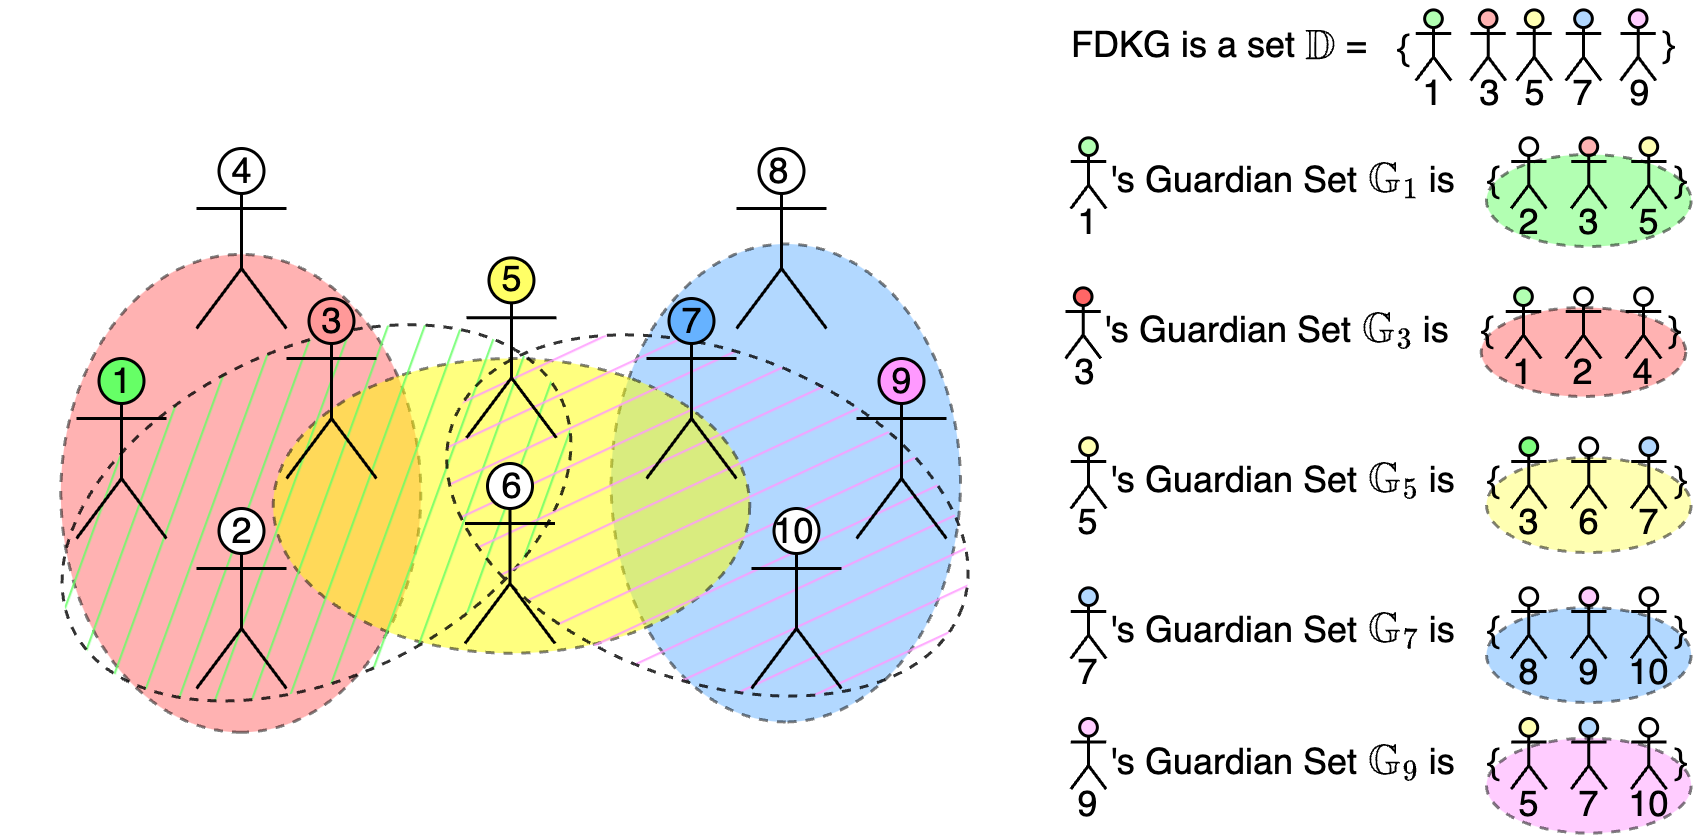
\includegraphics[width=\textwidth]{FDKG.png}
    \caption{Federated Distributed Key Generation}
    \label{fig:FDKG}
\end{figure}

The FDKG process for each participating party unfolds as follows:

\begin{enumerate}
    \item \textbf{Party $P_1$}:
        \begin{itemize}
            \item Chooses Guardian Set $\mathbb{G}_1 = \{P_2, P_3, P_5\}$.
            \item Samples a random polynomial $f_1(X) \in_R \mathbb{Z}_q[X]$, computes decryption key $d_1 = f_1(0)$.
            \item Distributes $d_1$ among $\mathbb{G}_1$, yielding shares $\PartialDecryptionKeyShare{1}{2}, \PartialDecryptionKeyShare{1}{3}, \PartialDecryptionKeyShare{1}{5}$.
        \end{itemize}

    \item \textbf{Party $P_3$}:
        \begin{itemize}
            \item Chooses Guardian Set $\mathbb{G}_3 = \{P_1, P_2, P_4\}$.
            \item Samples $f_3(X)$, computes $d_3$, and distributes it among $\mathbb{G}_3$, resulting in shares $\PartialDecryptionKeyShare{3}{1}, \PartialDecryptionKeyShare{3}{2}, \PartialDecryptionKeyShare{3}{4}$.
        \end{itemize}

    \item \textbf{Party $P_5$}:
        \begin{itemize}
            \item Chooses Guardian Set $\mathbb{G}_5 = \{P_3, P_6, P_7\}$.
            \item Samples $f_5(X)$, computes $d_5$, and distributes it among $\mathbb{G}_5$, producing shares $\PartialDecryptionKeyShare{5}{3}, \PartialDecryptionKeyShare{5}{6}, \PartialDecryptionKeyShare{5}{7}$.
        \end{itemize}

    \item \textbf{Party $P_7$}:
        \begin{itemize}
            \item Chooses Guardian Set $\mathbb{G}_7 = \{P_8, P_9, P_{10}\}$.
            \item Samples $f_7(X)$, computes $d_7$, and distributes it among $\mathbb{G}_7$, resulting in shares $\PartialDecryptionKeyShare{7}{8}, \PartialDecryptionKeyShare{7}{9}, \PartialDecryptionKeyShare{7}{10}$.
        \end{itemize}

    \item \textbf{Party $P_9$}:
        \begin{itemize}
            \item Chooses Guardian Set $\mathbb{G}_9 = \{P_5, P_7, P_{10}\}$.
            \item Samples $f_9(X)$, computes $d_9$, and distributes it among $\mathbb{G}_9$, resulting in shares $\PartialDecryptionKeyShare{9}{5}, \PartialDecryptionKeyShare{9}{7}, \PartialDecryptionKeyShare{9}{10}$.
        \end{itemize}
\end{enumerate}

In a traditional DKG protocol, the minimal set of parties needed to achieve Decipherability would be \(\{P_1, P_3, P_5, P_7, P_9 \}\). However, with the FDKG approach and the use of Guardian Sets, this minimum set is reduced to \(M = \{P_3, P_5, P_6\}\), demonstrating the protocol's efficiency in reducing the number of participants required for successful decryption.

\paragraph{Decipherability}
The set $M$ ensures Decipherability because shares $\PartialDecryptionKey{3},\PartialDecryptionKey{5},\PartialDecryptionKey{6}$ are published directly by those parties, whereas \PartialDecryptionKey{1} is recoverable by shares of \(\{P_3, P_5\}\) and \PartialDecryptionKey{9} is recoverable by shares of \(\{P_5, P_7\}\).

\paragraph{Privacy}
Privacy in the FDKG system is compromised when all parties from any Decipherability set collude. In this example, if all parties \(\{P_3, P_5, P_6\}\) collude, they can collectively reconstruct the secret \DecryptionKey{} and therefore decrypt each individual ballot \Ballot{i}.


\section{Experimental Results}

This section evaluates our voter-to-voter Internet voting protocol experimentally, focusing on proving times and message sizes for two prominent proving protocols: Plonk and Groth16, as implemented in the \texttt{snarkjs} WebAssembly (WASM) framework. The execution time for solving the Discrete Logarithm Problem (DLP) in the offline tally phase was also assessed. These experiments were conducted on a MacBook Pro with an Apple M1 Pro processor and 16GB of RAM.

\paragraph{Proving Time}

Table~\ref{table:proving-time} presents the time taken to generate a zkSNARK proof for each message using Groth16 and Plonk. The results indicate a significant performance difference between the two, with Groth16 showing superior efficiency. Notably, during the FDKG phase, Groth16 required a maximum of 2.414 seconds for a 3-of-4 configuration, compared to Plonk's 146.026 seconds for the same setup.


\begin{table}[!ht]
    \centering
    \begin{tabular}{|c|c|c|c|c|c|c|}
    \hline
        \multirow{2}{*}{\textbf{\shortstack{Proving\\ System}}} & \multicolumn{3}{|c|}{\textbf{FDKG}}  & \multirow{2}{*}{\textbf{\shortstack{Encrypt\\ Ballot}}} & \multirow{2}{*}{\textbf{\shortstack{Partial\\ Decryption}}} & \multirow{2}{*}{\textbf{\shortstack{Partial Decryption\\ Share}}} \\ 
        \cline{2-4}
        & \textbf{1 of 2} & \textbf{2 of 3} & \textbf{3 of 4} & &  &  \\ 
        \hline
        \textbf{Groth16} & 1.388 s & 2.135 s & 2.414 s & 0.747 s & 0.619 s & 0.580 s/share \\ 
        \hline
        \textbf{Plonk} & 67.753 s & 71.902 s & 146.026 s & 16.822 s & 16.543 s & 8.137 s/share \\ 
        \hline
    \end{tabular}
    \caption{Proving Time}
    \label{table:proving-time}
\end{table}

\paragraph{Message Size}

Table~\ref{table:message-size} details the message sizes required in each round of the protocol. Messages using Groth16 are smaller due to their proofs comprising only 3 elliptic-curve points, whereas Plonk-based proofs require 9 points and 6 scalars \cite{gabizonPLONKPermutationsLagrangebases2019}.

\begin{table}[!ht]
    \centering
    \begin{tabular}{|c|c|c|c|c|c|c|}
    \hline
        \multirow{2}{*}{\textbf{\shortstack{Proving\\ System}}} & \multicolumn{3}{|c|}{\textbf{FDKG}}  & \multirow{2}{*}{ \textbf{\shortstack{Encrypt\\ Ballot}}} & \multirow{2}{*}{\textbf{\shortstack{Partial\\ Decryption}}} & \multirow{2}{*}{\textbf{\shortstack{Partial Decryption\\ Share}}} \\ 
        \cline{2-4}
        & \textbf{1 of 2} & \textbf{2 of 3} & \textbf{3 of 4} & &  &  \\ 
        \hline
        \textbf{Groth16} & 1152 B & 1568 B & 1984 B & 512 B & 576 B & 768 B/share \\ \hline
        \textbf{Plonk} & 1472 B & 1888 B & 2304 B & 832 B & 896 B & 1088 B/share \\ \hline
    \end{tabular}
    \caption{Sizes of the Messages in Each Round}
    \label{table:message-size}
\end{table}

\paragraph{Discrete Logarithm Problem (DLP)}

A critical part of the offline tally in our protocol involves solving the DLP to extract the number of votes for each candidate. Although typically infeasible, the DLP can be solved through exhaustive search for a small number of voters. Using the method described in \cite{haoAnonymousVotingTworound2010}, we extracted each $x_i$ from the final output point $M$. 

Figure~\ref{fig:dlog-search} demonstrates that solving the DLP follows a power-law relation \( Y = aX^b \), with \( b \) varying linearly with the number of options. This finding suggests that while the time to solve DLP is linear with the number of voters, it grows exponentially with the number of candidates, posing scalability challenges in larger elections.

\begin{figure}[H]
    \centering
    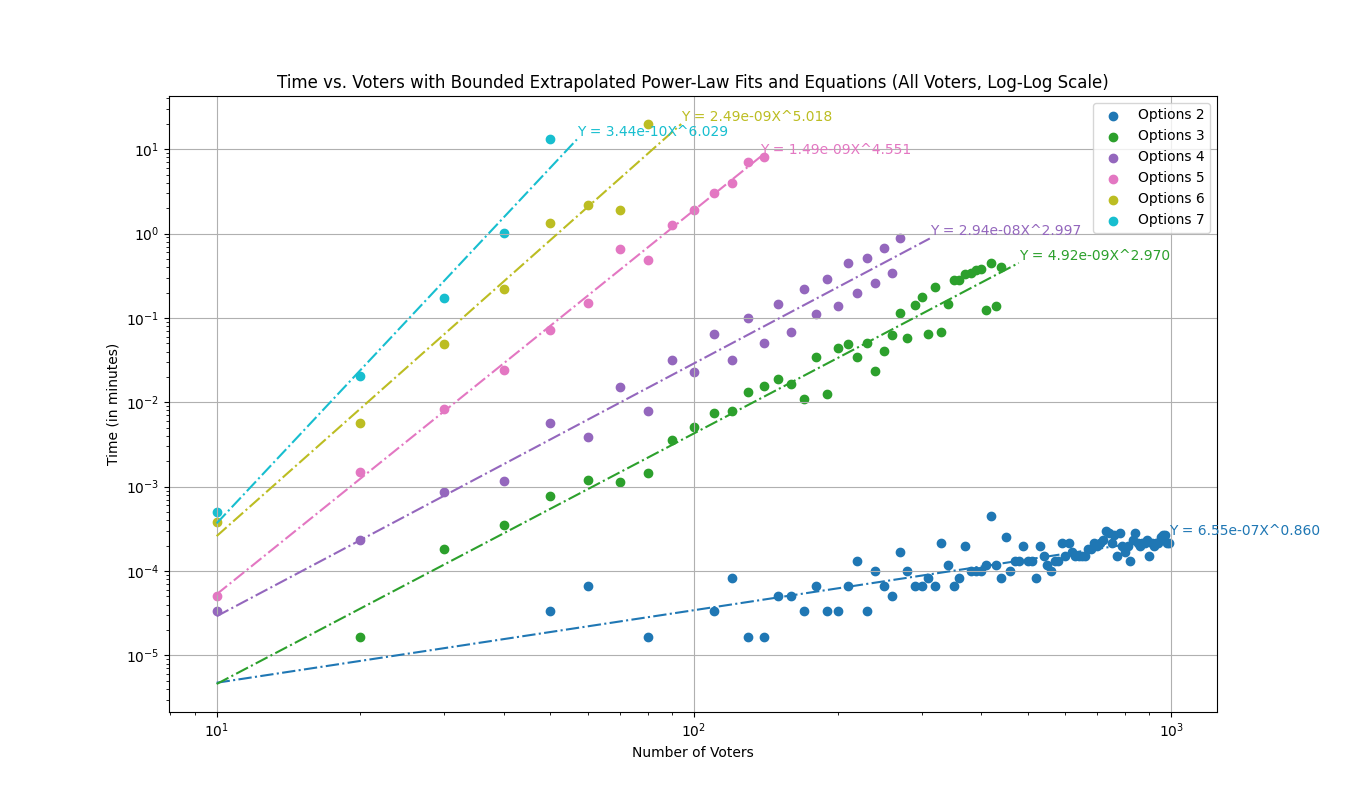
\includegraphics[width=\textwidth]{dlog-search-time.png}
    \caption{Time required to solve DLP with respect to the number of candidates and number of voters (log-log scale).}
    \label{fig:dlog-search}
\end{figure}


\section{Discussion}

Our work introduces a robust voting protocol that eliminates reliance on centralized entities and demonstrates resilience against node unavailability. The Federated Distributed Key Generation (FDKG) represents our principal innovation, extending traditional Distributed Key Generation (DKG) methods. FDKG uniquely allows for key reconstruction by parties within their Guardian sets, in addition to those participating in the original DKG. This generalization of DKG, where standard DKG equates to a 0-of-k FDKG protocol, significantly enhances protocol robustness by minimizing decipherability sets and maintaining privacy, with these sets including the network's most trusted parties.

The protocol's resilience is particularly valuable in contexts with uncertain network reliability and participant availability, ensuring secure and uninterrupted voting processes. Future research might involve simulating real-world trust dynamics in communities to assess the protocol's applicability \cite{healdMathematicalDescriptionTrust2019}.

However, implementing zkSNARKs for message certification introduces trade-offs between setup complexity and computational efficiency. Trusted setup ceremonies, such as those used in Groth16 \cite{grothSizePairingbasedNoninteractive2016}, offer greater efficiency compared to transparent, trustless setups like Plonk \cite{gabizonPlonkPermutationsLagrangebases2019a}. Our experiments indicated that, on a high-end personal computer, Groth16's proving time per message ranged from 1-3 seconds, while Plonk required 16-145 seconds. Although trusted setups entail strong assumptions, they are a one-time requirement and can be reused in future votings, a common practice in zkSNARK-based protocols.

A critical aspect of our protocol is the offline tally, reliant on solving the Discrete Logarithm Problem (DLP). The complexity of this task follows a power-law \( Y = aX^b \), with \( X \) proportional to the number of voters and \( b \) increasing with candidate count, indicating linear growth with voter numbers and exponential growth with candidate numbers. Addressing this scalability challenge could be a focus of future enhancements, potentially through more efficient algorithms.

Two deployment options for our protocol are proposed (see Figure~\ref{fig:stack-bc}): as a peer-to-peer application using IPFS\footnote{IPFS, An open system to manage data without a central server, \url{https://ipfs.tech/}} and Wesh Network\footnote{Wesh Network, Asynchronous mesh network protocol powered by Berty Technologies’ non-profit organisation, \url{https://wesh.network/}}, or as a smart contract on public blockchains, employing ERC-4337~\cite{ERC4337AccountAbstraction} to centralize voting costs under a single paymaster (e.g., organiser), allowing gasless voting for participants.

We have made our protocol's implementation in TypeScript and Golang open-source, facilitating widespread deployment and enhancing accessibility. The codebase is available at \url{https://github.com/stanbar/v2v-private-voting}.

Optimization avenues include improving proof times and sizes by batching proofs or reformulating them into more efficient Sigma Proofs. Another path involves on-chain implementation with gasless transactions, leveraging ERC-4337's paymaster concept.

\begin{figure}[H]
    \centering
    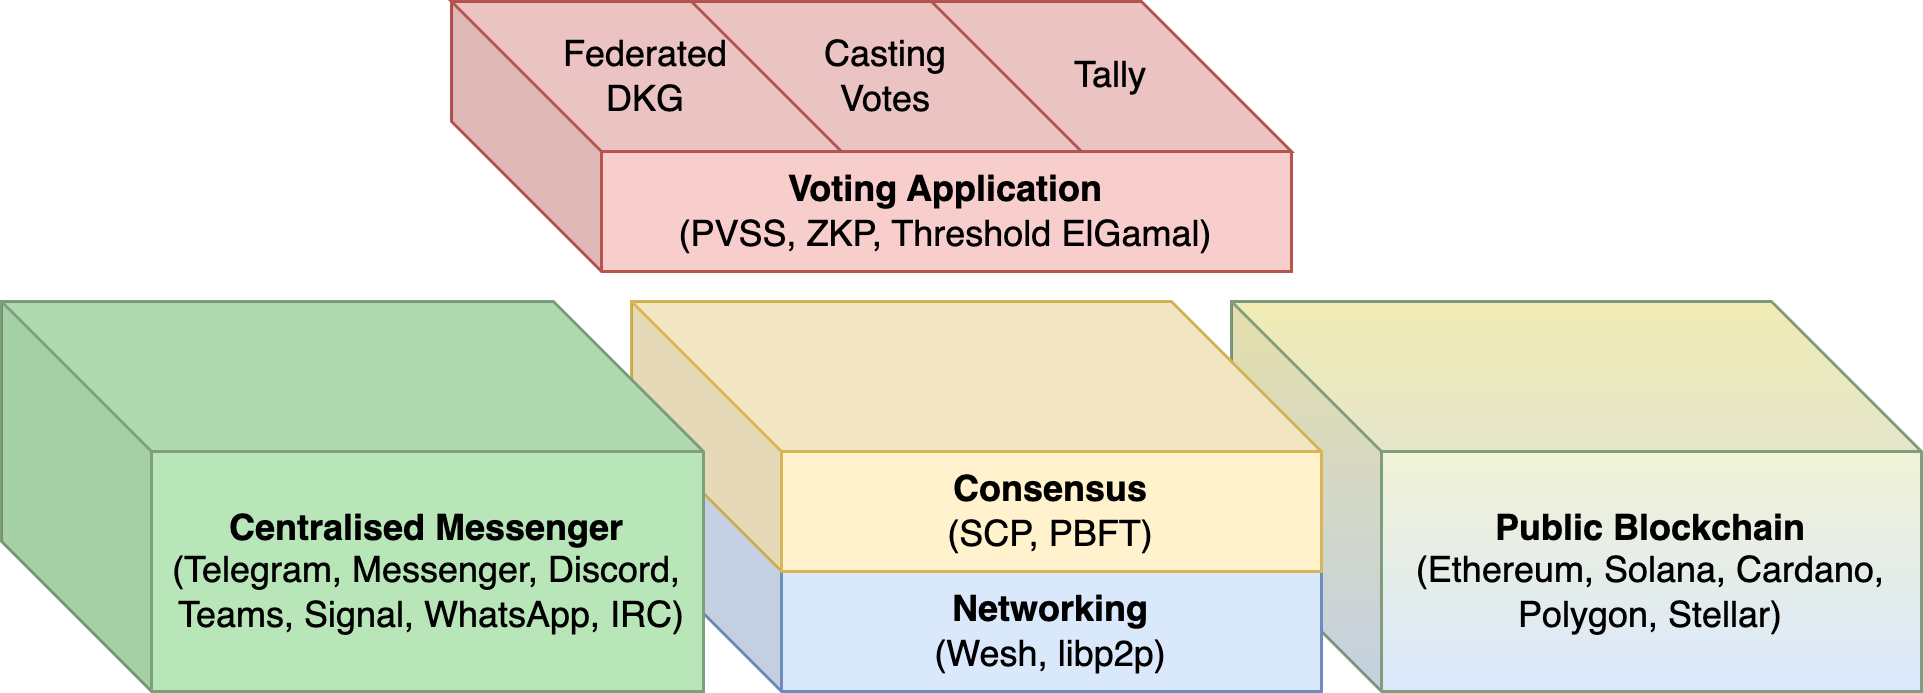
\includegraphics[width=\textwidth]{stack-bc.png}
    \caption{Architecture of the system.}
    \label{fig:stack-bc}
\end{figure}

\section{Conclusion}
This paper presents a voter-to-voter Internet voting protocol based on Federated Distributed Key Generation (FDKG), which significantly enhances the robustness and flexibility of Internet voting. FDKG achieves this by allowing key reconstruction by guardian sets, a feature that not only strengthens the robustness of the system against node unavailability, but also preserves privacy by relying on the most trusted parties in a network.

The practical applications of this protocol are many and powerful. It is particularly suited to small-scale voting environments such as local elections, NGO decision-making and corporate board resolutions. However, its adaptability also makes it a viable option for decentralised governance models in smart cities and DAOs, where secure and transparent voting is paramount. In addition, the protocol's scalability and privacy features make it a promising candidate for larger-scale implementations, such as regional or national elections, where traditional voting methods face logistical and security challenges.

The protocol faces challenges in terms of computational requirements and scalability, particularly for large-scale applications. Future research should focus on optimising zkSNARKs for efficiency and exploring scalable cryptographic solutions.

Looking ahead, we envision two primary deployment scenarios for our protocol: as a standalone peer-to-peer application utilizing open-source tools like IPFS and Wesh Network, or as a smart contract on public blockchains with gasless transactions enabled by the ERC-4337 standard. This flexibility in deployment options, coupled with our open-source implementation in TypeScript and Golang, underscores our commitment to accessibility and adaptability in various electoral contexts.

In conclusion, our protocol represents a meaningful step forward in the evolution of Internet voting systems. By embracing decentralization, enhancing security, and prioritizing privacy, we aim to contribute to the development of more resilient, trustworthy, and inclusive voting mechanisms in the digital age. As we continue to refine and optimize our protocol, we remain focused on the broader goal of modernizing democratic processes and empowering communities with reliable and accessible voting technologies.

\section{Acknowledgments}
We gratefully acknowledge Lev Soukhanov for his crucial role in designing the voting protocol and the Delendum team for their support and valuable insights during our research and development fellowship.

\bibliographystyle{IEEEtran}
\bibliography{bibliography}

\end{document}